\documentclass[12pt,a4paper]{ctexart}
\usepackage{amsmath}
\usepackage{amssymb}
\usepackage{graphicx}
\usepackage{float}
\usepackage{geometry}
\usepackage{subcaption}
\usepackage{booktabs}
\usepackage{array}
\usepackage{listings}
\usepackage{xcolor}
\usepackage{hyperref}
\geometry{a4paper, margin=1in}

\lstset{
    basicstyle=\ttfamily\footnotesize,
    keywordstyle=\color{blue},
    commentstyle=\color{gray},
    stringstyle=\color{red},
    numbers=left,
    numberstyle=\tiny\color{gray},
    stepnumber=1,
    numbersep=5pt,
    backgroundcolor=\color{white},
    showspaces=false,
    showstringspaces=false,
    showtabs=false,
    frame=single,
    tabsize=2,
    captionpos=b,
    breaklines=true,
    breakatwhitespace=false
}

% 设置中文字体为楷体
\setCJKmainfont{KaiTi} % 设置主字体为楷体
\setCJKsansfont{KaiTi} % 设置无衬线字体为楷体
\setCJKmonofont{KaiTi} % 设置等宽字体为楷体

\title{HW2：螺丝计数分析}
\author{李青雅 523030910004 电院2301}
\date{\today}

\begin{document}
\maketitle
\newpage
\tableofcontents % 生成目录
\newpage

\section{任务说明}

本次作业要求对俯视视角下的螺丝图像进行检测、分类与计数。输入是一个包含多张测试图像的文件夹，输出必须包括一个 \texttt{result.npy} 文件和一个 \texttt{time.txt} 文件。其中，\texttt{result.npy} 需要通过 \texttt{numpy.load(..., allow\_pickle=True).item()} 加载为字典，键为图像文件名去掉后缀后的 stem，值为长度为 5 的列表，顺序固定为
\[
[Type\_1, Type\_2, Type\_3, Type\_4, Type\_5].
\]

作业说明允许使用传统机器视觉方法，也允许使用深度学习方法。围绕这一要求，我一共做了三轮逐步收敛的探索：
\begin{itemize}
    \item 方法一：在 \texttt{method1\_abandoned} 中尝试用传统图像处理先自动裁出单个螺丝，再做后续分类准备；
    \item 方法二：在 \texttt{method2\_abandoned} 中尝试用五类 YOLO 直接完成整图检测与计数；
    \item 方法三：在 \texttt{code} 中采用当前最终主方案，即“单类 YOLO 检测 + 裁剪 + 分类器”的两阶段方法。
\end{itemize}

本报告严格按照作业要求，从“算法设计与流程”“实验与调优细节”“结果分析与局限性”三个角度描述三种方法，并客观分析每一阶段成功和失败的原因。

更多作者的心路历程和探索过程都在这份报告里了，这个报告不是AI写的，孩子做这个作业做得太憋屈了。

\section{总体探索路线}

这次作业的难度不只是“识别螺丝”，而是要在数据集十分有限，而图像的背景有干扰、螺丝数量较多、有两种螺丝长得很像以及一种螺丝是另一种螺丝的加长版等条件下，稳定输出五类螺丝的数量。由于数据规模较小，而且最终评分直接针对计数结果，因此我没有一次就得到满意方案，而是经历了以下逐步调整的过程：
\begin{enumerate}
    \item 首先尝试传统图像处理，希望先把单颗螺丝裁出来，减少人工标注工作量；
    \item 发现传统裁剪在背景格线、金属反光和粘连区域上不稳定后，转而尝试端到端五类检测；
    \item 进一步发现端到端五类检测在小数据集上验证指标较高，但真实计数效果并不稳定，于是改用更符合当前数据条件的两阶段方案：先检测，再分类。
\end{enumerate}

这三种方法并不是完全割裂的，而是一个我不断探索、逐步定位瓶颈、不断修正问题表述方式的过程。方法一帮助我确认了传统图像处理的局限；方法二帮助我确认了整图检测的方向是对的；方法三则在保留整图检测优点的同时，把细粒度分类从检测器中解耦出来，成为当前最合理的工程实现。

\section{方法一：传统图像处理自动裁剪方案}

\subsection{算法设计与流程}

方法一属于传统图像处理方案，目标不是直接输出最终五类计数，而是先通过边缘检测等方式生成候选螺丝 crop，然后这些crop要么再尝试其他的传统方法分类（比如二值图像面积）或者是SVM等学习的分类器。其基本流程如下：
\begin{enumerate}
    \item 将输入图像转为灰度图；
    \item 使用 CLAHE 增强局部对比度；
    \item 使用高斯滤波平滑噪声；
    \item 采用自适应阈值进行前景分割；
    \item 利用形态学开闭运算去掉小噪声并连接断裂区域；
    \item 在部分情况下尝试使用距离变换与 watershed 分离粘连目标；
    \item 提取连通域外接矩形并将其裁成小图。
\end{enumerate}

这一方法的核心出发点是：如果能较稳定地把单颗螺丝从大图中切出来，那么后续工作就只需要面对一批 crop，而不必直接在整图上逐个标注目标。

\subsection{实验与调优细节}

方法一对应的代码和数据主要位于 \texttt{method1\_abandoned} 目录。实验时使用的是 Homework 1 中完成透视矫正后的俯视图像。为了让裁剪结果更完整，我主要围绕以下参数反复试验：
\begin{itemize}
    \item CLAHE 的 \texttt{clipLimit} 与 \texttt{tileGridSize}；
    \item 高斯滤波核大小；
    \item 自适应阈值的窗口大小和常数项；
    \item 形态学开运算、闭运算的核大小；
    \item 是否使用 watershed 进一步分离疑似粘连区域。
\end{itemize}

这些参数的选定方式主要依赖于对裁剪结果的直接观察：如果背景保留过多，就收紧阈值或加强形态学操作；如果螺丝被裁断或碎裂，就放松阈值或尝试更弱的后处理。

图 \ref{fig:method1_cases_main} 展示了方法一中出现的几类典型 crop 结果。

\begin{figure}[H]
    \centering
    \begin{subfigure}[b]{0.31\textwidth}
        \centering
        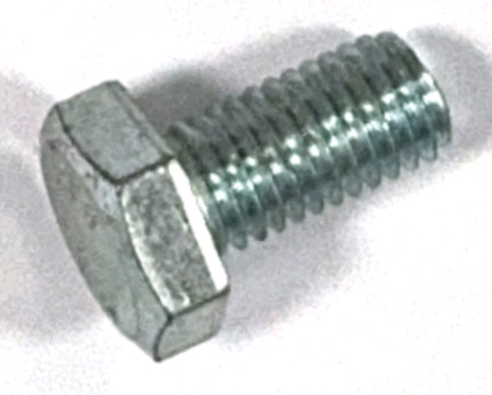
\includegraphics[width=\textwidth]{../submission/code/data/crops_raw/unlabeled/top01_obj_010.png}
        \caption{较成功的 crop}
    \end{subfigure}
    \hfill
    \begin{subfigure}[b]{0.31\textwidth}
        \centering
        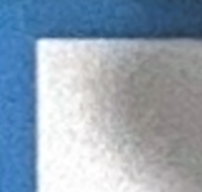
\includegraphics[width=\textwidth]{../submission/code/data/crops_raw/unlabeled/top10_obj_096.png}
        \caption{误裁到背景格线}
    \end{subfigure}
    \hfill
    \begin{subfigure}[b]{0.31\textwidth}
        \centering
        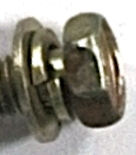
\includegraphics[width=\textwidth]{../submission/code/data/crops_raw/unlabeled/top02_obj_016.png}
        \caption{只截到螺丝局部}
    \end{subfigure}
    \caption{方法一中自动裁剪的典型结果}
    \label{fig:method1_cases_main}
\end{figure}

\subsection{结果分析与局限性}

方法一的结果并不理想。虽然在少量图像上能够裁出看起来比较完整的螺丝 crop，但整体上存在如下问题：
\begin{itemize}
    \item 容易将彩色田字格背景或背景纹理误当作目标；
    \item 容易只截取到螺丝的一部分，导致后续分类信息缺失，并且直接导致螺丝数量不准；
    \item 金属高光，螺纹形态和阴影会使同一颗螺丝在二值图中断裂，进而被切成多个碎片；
    \item 同一组形态学参数无法同时适应不同图像中的照明变化以及螺丝阴影。
\end{itemize}

从作业要求看，方法一虽然没有直接完成整图计数，只是为后续建数据集做准备，因此即便能生成一部分 crop，也很难作为最终提交方案。其失败的根本原因在于：本数据集中的螺丝边缘不够清晰，二阶导不够大和金属反光太强，传统图像处理基本上不可能在所有图上给出稳定而干净的候选区域。到此，我基本上确认了需要转向深度学习方法，上学期学的数字图像处理方法只有可能作为图像预处理，我还是需要直接在整图上进行检测和分类。

\section{方法二：五类 YOLO 端到端检测方案}
在传统图像处理方法上失败了，于是我很轻易地想到使用YOLO。但是面临着同样的问题：数据集太小了，只有十张图像。我当初就是因为数据集太小所以才没有直接考虑学习的方法，但是在标数据的时候，惊讶地发现AI自动标注的能力还比较好，所以考虑直接把五类螺丝都标出来，在整图上训练一个五类检测器。这样就直接面向作业最终目标了：整图输入、整图检测、五类计数输出。

\subsection{算法设计与流程}

方法二属于深度学习检测方案。它直接把五类螺丝都作为检测类别，在整张图像上同时完成定位和分类。整体流程如下：
\begin{enumerate}
    \item 在整张图像上手工标注每颗螺丝的边界框与类别，这里我使用的标注工具是trexlabel；
    \item 将标注导出为 YOLO 检测格式；
    \item 构建训练集和验证集；
    \item 使用预训练的 YOLO 模型进行五类检测微调；
    \item 推理时对整图输出检测框与类别；
    \item 按类别统计检测框数量并生成最终计数结果。
\end{enumerate}

与方法一相比，方法二已经直接面向作业最终目标：整图输入、整图检测、五类计数输出。

\subsection{实验与调优细节}

我使用手工标注的数据对 YOLO 进行了五类微调，采用的基础模型为 \texttt{yolo11n.pt}。一开始尝试使用了\texttt{yolo11s.pt}，但是我的电脑只能用cpu跑，后者模型对我来说不够轻量。训练时的主要设置为：
\begin{itemize}
    \item 训练轮数：100 epoch；
    \item 输入尺寸：1280；
    \item batch size：2；
    \item 训练设备：CPU；
    \item 数据增强：使用了 YOLO 默认的数据增强，包括缩放、平移、翻转与 mosaic。
\end{itemize}

数据划分上，我使用了 10 张已标注图像，其中 8 张用于训练，2 张用于验证。图 \ref{fig:method2_annotation_main} 给出了方法二中五类标注数据的示例。

\begin{figure}[H]
    \centering
    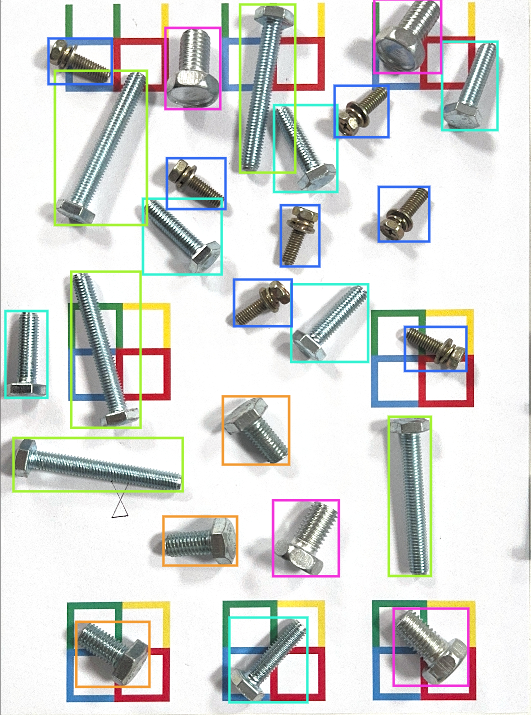
\includegraphics[width=0.88\textwidth]{../submission/code/dataset/example.png}
    \caption{方法二中五类 YOLO 标注数据示例}
    \label{fig:method2_annotation_main}
\end{figure}

这里其实是网站上的AI半自动标注，也就是我先框出一个矩形，然后AI可以自动识别出所有的矩形；而且它的识别效果非常好，每一个单独的螺丝都识别出来了，矩形框基本上是紧贴着螺丝的，而且即使螺丝之间距离很近也没有合并矩形框；背景里的格线和纹理，以及干扰的黑三角基本上没有被误识别成螺丝。所以标注量主要在手动把框出来的螺丝分类。

根据训练日志，方法二在极小验证集上可以得到较高的检测指标，例如：
\begin{itemize}
    \item Precision(B) $\approx 0.99$；
    \item Recall(B) $\approx 1.00$；
    \item mAP50(B) $\approx 0.995$；
    \item mAP50-95(B) $\approx 0.991$。
\end{itemize}

这些数字在表面上看非常好，但后续样例图像上的真实计数效果并没有达到相同水平。

\subsection{结果分析与局限性}

根据作业说明，两张样例图像的真实结果为：
\[
\text{01}: [6, 3, 4, 2, 4], \qquad
\text{02}: [14, 1, 1, 8, 1].
\]

方法二给出的代表性预测结果为：
\[
\text{01}: [9, 3, 6, 2, 3], \qquad
\text{02}: [19, 2, 2, 6, 1].
\]

表 \ref{tab:method2_result_main} 给出了方法二在两张样例图像上的计数结果。

\begin{table}[H]
    \centering
    \caption{方法二在两张样例图像上的计数结果}
    \label{tab:method2_result_main}
    \begin{tabular}{c|c|c|c}
        \toprule
        图像 & 真值 & 预测值 & 绝对误差 \\
        \midrule
        01 & [6, 3, 4, 2, 4] & [9, 3, 6, 2, 3] & [3, 0, 2, 0, 1] \\
        02 & [14, 1, 1, 8, 1] & [19, 2, 2, 6, 1] & [5, 1, 1, 2, 0] \\
        \bottomrule
    \end{tabular}
\end{table}

方法二的主要问题有三点：
\begin{itemize}
    \item 数据量太小，训练集只有 8 张图像，五类检测很容易过拟合；
    \item 验证集只有 2 张图像，导致验证指标过于乐观；
    \item 细粒度类别差异直接压在检测器上学习，在小数据条件下难度过高。
\end{itemize}

但是我还是不死心，搜了一下有没有做小样本检测的论文。由于作业要求对准确率要求实在是太高了，螺丝个数误差大于等于两个就没分。所以我抛弃了度量学习和元学习等经典模型，而是找到了当前SOTA：使用Transformer + 小样本的PrototypeFormer。论文链接：https://arxiv.org/pdf/2310.03517。这篇论文是2024年的AAAI，但是很遗憾并没有开源，而我一个人根据论文搭起整个模型实在是太困难了，所以我就放弃了这个方向。

因此，方法二虽然方向上更贴合作业要求，但在当前数据规模下并没有产生足够稳定的泛化效果。

\section{方法三：单类 YOLO 检测加分类器的两阶段方案}
既然前两个方法都失败了，我也在着手考虑新的方法。这个时候忽然想到在方法二里用的AI标注，虽然不能直接标五类，但它能帮我标出所有的螺丝候选框。也就是说，我可以先训练一个单类检测器，把所有的螺丝都找出来，不区分类别；然后再对每个检测框裁剪出一个 crop，单独训练一个分类器来区分这五类螺丝。这样就把“定位”和“细粒度分类”拆开了，每个子任务的难度都降低了很多，更适合当前样本量较小的场景。

\subsection{算法设计与流程}

方法三是当前最终主方案，代码位于 \texttt{code} 中。它采用的是深度学习两阶段方法：先做单类检测，再做细粒度分类。整体流程如下：
\begin{enumerate}
    \item 使用单类 YOLO 检测器定位所有疑似螺丝，只判断“是不是螺丝候选框”；
    \item 对每个检测框裁剪出一个 crop；
    \item 用分类器将 crop 分到 \texttt{Negative}、\texttt{Type\_1}、\texttt{Type\_2}、\texttt{Type\_3}、\texttt{Type\_4}、\texttt{Type\_5} 六类之一；
    \item 推理时忽略 \texttt{Negative}，仅统计五类螺丝数量；
    \item 将结果按作业要求写入 \texttt{result.npy}，并将总耗时写入 \texttt{time.txt}。
\end{enumerate}

这一方法的关键思想是把“定位”和“细粒度分类”拆开。单类检测器只需要学会把螺丝从背景中找出来，而分类器只需要在小图上区分螺丝类型。与方法二相比，它显著降低了每个子任务的难度，更适合当前样本量较小的场景。

方法三对应的主程序入口是 \texttt{code/run.py}，可以直接满足作业对于输入输出格式的要求：
\begin{lstlisting}[language=bash, caption={方法三统一入口}]
python run.py --data_dir /path/to/test_images --output_path ./result.npy --output_time_path ./time.txt
\end{lstlisting}

\subsection{实验与调优细节}

\paragraph{1. 检测器数据集与训练}
做检测器的时候甚至想过能不能外接那个模型的AI标注，因为它们效果确实好，再串联把他们的输出作为分类器的输入，应该效果会非常好。但是后来考虑到作业要求的严苛性，还是决定自己训练一个单类检测器。

方法三的检测器训练数据来自 \texttt{dataset\_oneclass}。我先使用 \texttt{prepare\_detector\_split.py} 构建单类 YOLO 数据集，再使用 \texttt{train\_detector.py} 训练检测器。最终检测器的主要训练配置为：
\begin{itemize}
    \item 基础模型：\texttt{yolo11n.pt}；
    \item 输入尺寸：640；
    \item batch size：2；
    \item 设备：CPU；
    \item dataloader workers：0；
    \item Ultralytics 默认早停参数：\texttt{patience=100}。
\end{itemize}


在对多个单类 detector run 做了可视化比较之后，我最终没有继续使用指标更高的 \texttt{screw\_oneclass6}，而是选用了实际检测效果更稳定的 \texttt{screw\_oneclass3}。这一 run 的训练配置记录在 \texttt{hw22/submission/code/models/detector\_runs/screw\_oneclass3/args.yaml} 中，总训练轮数为 80 个 epoch。根据 \texttt{results.csv} 的记录，最佳权重对应第 76 个 epoch，验证集指标为：
\begin{itemize}
    \item Precision(B) = 1.00000；
    \item Recall(B) = 0.99806；
    \item mAP50(B) = 0.99500；
    \item mAP50-95(B) = 0.87433。
\end{itemize}

图 \ref{fig:method3_detector_train_main} 左图给出了 \texttt{screw\_oneclass3} 的训练曲线，右图给出了该 run 自动统计得到的标签相关性图（\texttt{labels\_correlogram.jpg}）。从训练曲线可以看出，该 detector 在前 20 个 epoch 以后性能已经明显提升，在 40 个 epoch 之后逐渐进入稳定区间，并最终在第 76 个 epoch 达到最佳验证指标。右侧的标签相关性图则反映了训练数据中目标框的空间分布、宽高比例和共现关系：可以看到单类螺丝框的尺度分布相对集中，这说明使用单类检测器先学习“螺丝整体外形”是合理的；同时，不同图像中的目标密度和相邻框关系也较复杂，这恰好解释了为什么后续仍然会出现重复框、长螺丝被拆成两框等问题。也正因为如此，我最终选择 \texttt{screw\_oneclass3} 作为方法三检测器，不仅是看它的验证指标，更重要的是它在实际 detector-only 可视化中，在召回率、重复框数量和后续分类可用性之间达到了更好的平衡。

\begin{figure}[H]
    \centering
    \begin{subfigure}[b]{0.58\textwidth}
        \centering
        
\includegraphics[width=\textwidth]{../../hw22/submission/code/models/detector_runs/screw_oneclass3/results.png}
        \caption{\texttt{screw\_oneclass3} 训练过程曲线}
    \end{subfigure}
    \hfill
    \begin{subfigure}[b]{0.38\textwidth}
        \centering
        
\includegraphics[width=\textwidth]{../../hw22/submission/code/models/detector_runs/screw_oneclass3/labels_correlogram.jpg}
        \caption{训练集标签相关性图}
    \end{subfigure}
    \caption{方法三中最终采用的单类检测器 \texttt{screw\_oneclass3} 的训练过程与数据分布分析}
    \label{fig:method3_detector_train_main}
\end{figure}

\paragraph{2. 分类器数据集构建}
检测器训练完成后，我使用 \texttt{prepare\_classifier\_crops.py} 从单类标注框中裁出所有正样本，再手工将它们整理到 \texttt{Type\_1} 到 \texttt{Type\_5} 五个文件夹中。同时，我使用 \texttt{sample\_negative\_crops.py} 自动从背景区域补充一部分负样本，放入 \texttt{Negative} 类，以便让分类器学会拒绝非螺丝或低质量候选框。

在当前一版数据集中，分类器划分后的训练/验证样本数分别为：
\begin{itemize}
    \item 训练集：\texttt{Negative}=26，\texttt{Type\_1}=43，\texttt{Type\_2}=30，\texttt{Type\_3}=27，\texttt{Type\_4}=54，\texttt{Type\_5}=20；
    \item 验证集：\texttt{Negative}=6，\texttt{Type\_1}=11，\texttt{Type\_2}=7，\texttt{Type\_3}=7，\texttt{Type\_4}=13，\texttt{Type\_5}=5。
\end{itemize}

\paragraph{3. 分类器结构替换与训练}
一开始我的分类器使用的是 \texttt{ResNet18}。在实际端到端测试中，我发现仅使用 \texttt{ResNet18} 时，效果并不是很好，因此后续将分类器更换为 \texttt{EfficientNet-B0}。前者的参数量和计算量都不大，但是不能很好地区分螺丝，因为螺丝头部纹理，长度比例和细小螺纹槽都有所不同；而后者是更高效的神经网络，由于使用了MBConv、SE attention 和更系统的宽度/深度/分辨率联合缩放，更擅长提取细节特征。同时在训练脚本中加入了更适合小数据集的设置：
\begin{itemize}
    \item 输入尺寸由 224 调整到 256；
    \item 默认学习率设置为 \texttt{5e-4}；
    \item batch size 设置为 16；
    \item 加入类别权重，缓解类别不均衡；
    \item 加入 \texttt{label smoothing}；
    \item 加入 early stopping。
\end{itemize}

当前分类器 checkpoint 中记录的最优结果为：
\begin{itemize}
    \item 架构：\texttt{efficientnet\_b0}；
    \item 最佳验证精度：1.0000；
    \item 最佳验证损失：0.2709；
    \item 最佳 epoch：33。
\end{itemize}

\paragraph{4. 遇到的困难与解决过程}
方法三并不是一次就成功的，中间遇到了一堆问题：
\begin{itemize}
    \item \textbf{训练环境问题。} 最初直接按 \texttt{device=0} 训练会报 CUDA 不可用错误，不知道为什么我的1650无法使用，后来切换到 CPU 训练，并采用更轻量的 \texttt{yolo11n}，然后先跑一个epoch试试，使训练流程先稳定跑通。
    \item \textbf{分类器验证精度高，但端到端效果差。} 分类器在 crop 级验证集上可以达到很高精度，但实际整图计数并不理想。后来分析摸排发现，训练时使用的是人工标注框裁出的较干净 crop，而推理时输入的是检测器的输出，两者分布并不一致。然而后面我尝试使用检测器的输出框裁剪训练分类器，发现验证集上的分类精度反而下降了；可能是因为检测器本身效果就没有人家网站上效果好，所以用它的输出框裁剪训练数据反而引入了更多噪声。
    \item \textbf{误检框导致错误计数。} 为了解决这一问题，我在分类器中加入了 \texttt{Negative} 类，并补充了背景负样本，让分类器在第二阶段过滤掉明显不是目标的 crop。但是也不能加入过多和正常螺丝过于相似的负样本，比如这里长螺丝的前半部分和中螺丝很像，如果把它们也当作负样本加入训练，分类器就会直接漏检。
    \item \textbf{检测器重复框较多。} 在 detector-only 可视化时，常见问题是一颗螺丝被框两次（再次对长螺丝和中螺丝无语）。为此我一方面给检测器数据集中补充了空标签负样本图，另一方面在推理后处理里增加了基于 \texttt{IoU} 和包含关系的二次去重参数（\texttt{detector\_duplicate\_iou} 和 \texttt{detector\_duplicate\_containment}）。效果稍微好了一点，但仍然存在一些重复框。
    \item \textbf{阈值存在召回与重复框的折中。} 当 \texttt{conf} 设得太低时，重复框显著增多；当 \texttt{conf} 与去重阈值设得过严时，又会出现漏检。因此，方法三最终需要联合调节 \texttt{detector\_conf}、\texttt{detector\_iou}、\texttt{classifier\_min\_conf} 以及二次去重参数。
\end{itemize}

关于这里的一些参数，以下是我在调试过程中总结的一些经验和查阅的资料：
\begin{enumerate}
    \item detector\_conf：检测器置信度阈值，YOLO 只保留分数高于这个值的框。设低了：框更多，召回更高，但误检和重复框会增多；设高了：框更少，更干净，但容易漏检。
    \item detector\_iou：YOLO 自带 NMS 的 IoU 阈值，它决定“两个重叠框像到什么程度时，要不要压掉一个”。设低了：NMS 更狠，更容易去掉重复框；设高了：NMS 更松，会保留更多相近框。
    \item classifier\_min\_conf：分类器最小置信度阈值，检测框裁成 crop 后，分类器会给出六分类结果和分数；如果最高分类分数低于这个值，就直接忽略，不计数。设低了：更多 crop 会被计入，召回更高，但错分更多；设高了：只有分类器很有把握时才计数，但容易漏记。
    \item 二次去重参数：detector\_duplicate\_iou 和 detector\_duplicate\_containment：前者是检测后再做一次去重时使用的 IoU 阈值，如果两个框的 IoU 超过它，就认为可能是重复框，删掉低分那个；设低了：去重更狠；设高了：去重更松。后者是检测后再看“一个框是否几乎被另一个框包住”，如果小框大部分被大框覆盖，就认为是套娃重复框；设低了：更容易删掉这类套娃框；设高了：更保守，不轻易删。
\end{enumerate}

\begin{figure}[H]
    \centering
    \begin{subfigure}[b]{0.48\textwidth}
        \centering
        
\includegraphics[width=\textwidth]{../../hw22/submission/code/data/classifier_raw/unlabeled_positive/top01_obj_000.png}
        \caption{检测器裁出的正样本示例}
    \end{subfigure}
    \hfill
    \begin{subfigure}[b]{0.48\textwidth}
        \centering
        \includegraphics[width=\textwidth]{../../hw22/submission/code/data/classifier_split/train/Negative/neg02.png}
        \caption{分类器中的负样本示例}
    \end{subfigure}
    \caption{方法三中用于分类器训练的样本示例}
    \label{fig:method3_classifier_sample_examples}
\end{figure}


\paragraph{5. Debug 可视化}
为了定位方法三的问题，我分别保存了 detector-only 的可视化结果和最终两阶段推理可视化结果。图 \ref{fig:method3_debug_main} 左图展示了单类检测器在训练集图像上的输出框，右图展示了最终两阶段流程在样例图像上的分类与计数可视化。可以看到，方法三的主要困难不再是“完全找不到螺丝”，而是在“保召回”和“压重复框”之间寻找平衡。

\begin{figure}[H]
    \centering
    \begin{subfigure}[b]{0.48\textwidth}
        \centering
        
\includegraphics[width=\textwidth]{../../hw22/submission/code/detector_debug_vis/train/top01.png}
        \caption{单类检测器 debug 可视化}
    \end{subfigure}
    \hfill
    \begin{subfigure}[b]{0.48\textwidth}
        \centering
        \includegraphics[width=\textwidth]{../../hw22/submission/code/debug_vis/01_debug.png}
        \caption{两阶段最终推理 debug 可视化}
    \end{subfigure}
    \caption{方法三的 detector-only 与两阶段可视化结果}
    \label{fig:method3_debug_main}
\end{figure}

可以看到其实有的时候检测器的效果还是很好的，能够把大部分螺丝都框出来；但是偶尔会有重复框，主要是在长螺丝上，切割的话很容易切成中螺丝；并且还会把背景里的三角干扰识别成螺丝。而在端到端检测里，成功识别的螺丝都比较自信，但是也面临会把长螺丝前半截识别成中螺丝或者短螺丝。

\subsection{结果分析与局限性}

根据作业给出的两张样例图像真值：
\[
\text{01}: [6, 3, 4, 2, 4], \qquad
\text{02}: [14, 1, 1, 8, 1].
\]

方法三在默认参数下的早期结果是：
\[
\text{01}: [7, 4, 5, 8, 4], \qquad
\text{02}: [15, 1, 1, 9, 2].
\]
这一结果说明系统存在明显的过检和重复框问题。

在加入 \texttt{Negative} 类、将分类器切换到 \texttt{EfficientNet-B0}、并对检测与分类阈值进行一轮联合调参后，一组相对比较稳定的结果为：
\[
\text{01}: [6, 1, 5, 3, 3], \qquad
\text{02}: [13, 1, 1, 8, 0].
\]

与方法二相比，方法三在样例图像上的总体计数已经更接近真值。以作业给出的评分方式估算，方法二在两张图上的表现大约可折算为 45\%，而方法三这一组结果可提升到约 65\% 左右。这说明将任务拆成“检测 + 分类”两步是有效的。

不过，方法三目前仍有以下局限：
\begin{itemize}
    \item 分类器虽然在 crop 级验证集上达到很高精度，但端到端表现仍受 detector crop 分布影响；
    \item 当检测阈值较低时，重复框和误检会显著增多；
    \item 当去重和分类阈值过严时，又会出现漏检和漏记；
    \item 当前验证集仍然较小，结果可能偏乐观，泛化能力还需在更多图像上验证。
    \item 模型仍然无法区分长螺丝的前半部分和中螺丝，不管是检测器还是分类器都很容易把它们搞混。
    \item 限于时间，我没有做数据增强或者是生图造新数据。
\end{itemize}

整体而言，方法三已经明显优于前两种方法，但仍处在“可运行、可分析、可继续优化”的阶段，而不是完全收敛的最终最优解。

\section{三种方法的对比总结}

三种方法的特点可以概括如下：

\begin{table}[H]
    \centering
    \caption{三种方法的对比}
    \label{tab:three_methods_compare_main}
    \begin{tabular}{p{2.5cm}p{3.8cm}p{3.8cm}p{4.0cm}}
        \toprule
        维度 & 方法一：传统裁剪 & 方法二：五类 YOLO & 方法三：单类检测 + 分类器 \\
        \midrule
        方法类型 & 传统机器视觉 & 深度学习单阶段检测 & 深度学习两阶段方法 \\
        核心流程 & 图像处理后导出 crop & 整图检测并直接分类计数 & 先检测，再裁剪，再分类计数 \\
        主要优点 & 不依赖复杂训练 & 直接贴合作业目标 & 更适合小样本和细粒度类别 \\
        主要问题 & 背景误裁严重，crop 不稳定 & 小数据下过拟合明显 & 仍需处理重复框与阈值折中 \\
        当前结论 & 不适合作为最终方案 & 可作强基线，但泛化不足 & 是当前主方案，也是后续继续优化的方向 \\
        \bottomrule
    \end{tabular}
\end{table}

从实验逻辑上看，方法一失败在于在有限时间内传统方法难以应对复杂情况，这种分类计数问题本来就是神经网络的舒适区；方法二失败在于把过多难度压给了小数据条件下的单阶段检测器，要是数据足够多肯定没问题；方法三则通过拆分任务降低了学习难度，因此在当前条件下取得了最平衡的效果。

\section{代码与提交要求对应关系}

当前最终提交对应的是 \texttt{submission/code/} 目录。该目录已经按照作业说明组织，包含：
\begin{itemize}
    \item \texttt{run.py}：统一推理入口；
    \item \texttt{README.md}：环境、命令和数据准备说明；
    \item \texttt{requirements.txt}：依赖列表；
    \item \texttt{models/}：检测器与分类器权重；
    \item \texttt{scripts/}：数据准备、训练和可视化脚本；
    \item \texttt{src/}：核心推理代码。
\end{itemize}

方法三可以直接满足作业的三个关键接口要求：
\begin{enumerate}
    \item 输入目录通过 \texttt{--data\_dir} 指定；
    \item 输出 \texttt{result.npy} 和 \texttt{time.txt}；
    \item 程序结束时会在终端打印总处理时间。
\end{enumerate}

因此，从“逻辑清晰、算法完整、代码可运行、接口符合要求”的角度看，方法三已经具备作为正式提交方案的完整性。

\section{结论和感想}

本次作业我的的核心收获不只是得到一个能运行的计数程序，更重要的是明确了在小数据规模下，什么样的问题建模方式更合适；怎么去面对不同参数的权衡，怎么探索不同的方法。

方法一说明：传统图像处理难以在复杂背景和金属反光条件下稳定得到高质量 crop。方法二说明：虽然端到端五类检测在形式上最直接，但在小样本条件下很容易出现“验证指标高、真实计数不稳”的现象。方法三则通过“单类检测 + 裁剪分类”的两阶段设计，将任务拆成两个更容易学习的子问题，并通过加入 \texttt{Negative} 类、更换分类器、补充检测器负样本、增加二次去重和联合调阈值等方式，逐步解决了误检、重复框和细粒度分类不稳的问题。

从当前结果看，方法三已经是三种方案中最合理、最接近最终作业要求的实现。尽管它在样例图像上仍然存在漏检与重复框之间的权衡问题，但它已经具备清晰的调优方向：继续补充更贴近真实推理分布的 hard negative、扩大分类训练集、改进验证集划分方式，并进一步调节 detector 和 classifier 的协同阈值。也正因为经历了这三个阶段，本报告能够较完整地呈现一条从失败到修正、再到收敛的探索路径。

在这次作业中，我遇到了很多困难，很多连ai都无法解决的问题（也可能是我ai能力有限），于是自己看论文，找资料。期间还和同学讨论过，也想到了很多不一样的方法，比如外接网站，用滑动窗口和拼接图片来做数据增强，甚至是用生成模型来做数据增强。我也很清楚班上肯定有同学能把每一颗螺丝分出来，但是我已经尽我所能了，这已经是我尝试好几天的结果了。总之，这次作业虽然很难，我也基本上是骂骂咧咧写完的（笑）。但写完了之后我觉得非常有意义，也学到了很多东西。

\end{document}
